\section{Analysis}\label{sec:analysis}

\begin{proposition}[Predictive triggering is a rate-scaled margin]\label{prop:reduction}
On its positive-rate branch, the predictive rule in \eqref{eq:pred} is a reactive threshold with the time-varying pad $\rho(t)=T_h\hat r(t)$; its fallback pad is zero. Suppose that, on a monitored interval containing both threshold crossings, $M(t)=r(t_0-t)$ with an exact constant estimate $\hat r=r>0$, and that monitoring begins before either crossing. The predictive rule then fires $T_h$ seconds before $t_0$, while a fixed pad $\rho$ fires $\rho/r$ seconds before $t_0$. Thus, at one known constant rate, the fixed pad $\rho=T_h r$ reproduces the predictive trigger exactly. For a positive horizon and two distinct rates, no one fixed pad provides that same constant positive lead time at both rates.
\end{proposition}
\begin{proof}
The threshold identity on the positive-rate branch follows directly from \eqref{eq:pred}. Under the stated affine model, $M(t_0-L)=rL$. The predictive threshold $M=T_h r$ is therefore reached at $L=T_h$, and the fixed threshold $M=\rho$ at $L=\rho/r$; the monitoring assumption makes these the first threshold crossings. If $T_h>0$ and $r_1\ne r_2$, matching that lead at both rates would require both $\rho=T_h r_1$ and $\rho=T_h r_2$, which is impossible.
\end{proof}

\begin{proposition}[When lead time changes the recovery outcome]\label{prop:boundary}
Assume a predictive rule triggers $L\ge0$ seconds before $t_0$, while the unpadded reactive rule triggers at $t_0$. Then:
\begin{enumerate}
  \item if $\tau_r\le\delta$, both rules recover in time;
  \item if $\delta<\tau_r\le\delta+L$, only the predictive trigger recovers in time; and
  \item if $\tau_r>\delta+L$, neither rule recovers in time.
\end{enumerate}
\end{proposition}
\begin{proof}
By \eqref{eq:success}, the unpadded rule succeeds exactly when $t_0+\tau_r\le t_f$, or $\tau_r\le\delta$. The predictive rule succeeds exactly when $t_0-L+\tau_r\le t_f$, or $\tau_r\le\delta+L$. The three cases follow.
\end{proof}

\begin{corollary}[Necessary conditions for an advantage over fixed pads]\label{cor:factors}
Within the deadline-only model of Proposition~\ref{prop:boundary}, an earlier predictive trigger turns a recovery failure into success only in the middle band, which requires positive lead. Within the affine, exact-rate model of Proposition~\ref{prop:reduction}, a positive-horizon predictor can have a structural advantage over a \emph{single fixed pad across cases} only if the degradation rates vary: at one known constant rate, an equivalent fixed pad exists. These conditions are necessary within the stated models, not sufficient; estimation error and the joint distribution of rates, slack, and recovery times can still make a fixed pad preferable.
\end{corollary}

Figure~\ref{fig:mech} illustrates the timing argument.

\begin{figure}[tbp]
\centering
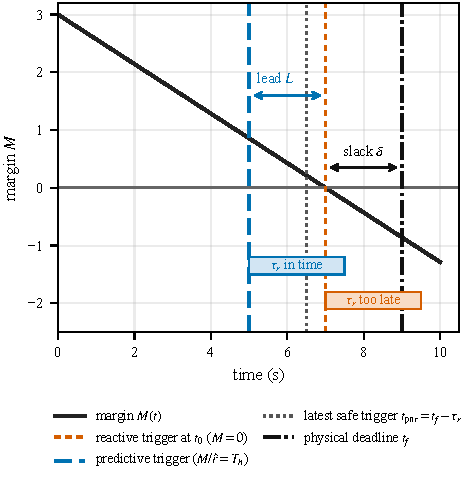
\includegraphics[width=0.72\linewidth]{fig_mechanism.pdf}
\caption{The unpadded reactive rule fires at margin expiry, while the predictive rule fires $L$ seconds earlier. The earlier trigger changes the recovery outcome only when $\delta<\tau_r\le\delta+L$.}
\label{fig:mech}
\end{figure}
